\documentclass[svgnames,11pt]{beamer}
\input{/home/tof/Documents/Cozy/latex-include/preambule_commun.tex}
\input{/home/tof/Documents/Cozy/latex-include/preambule_beamer.tex}
%\usepackage{pgfpages} \setbeameroption{show notes on second screen=left}
\author[]{Christophe Viroulaud}
\title{Puissance 4}
\date{\framebox{\textbf{Lang 08}}}
%\logo{}
\institute{Première - NSI}

\begin{document}
\begin{frame}
        \note{\fcolorbox{black}{red}{{\LARGE puissance4-annexe.zip}}}
    \titlepage
\end{frame}
\begin{frame}
    \frametitle{}

    \begin{center}
        \centering
        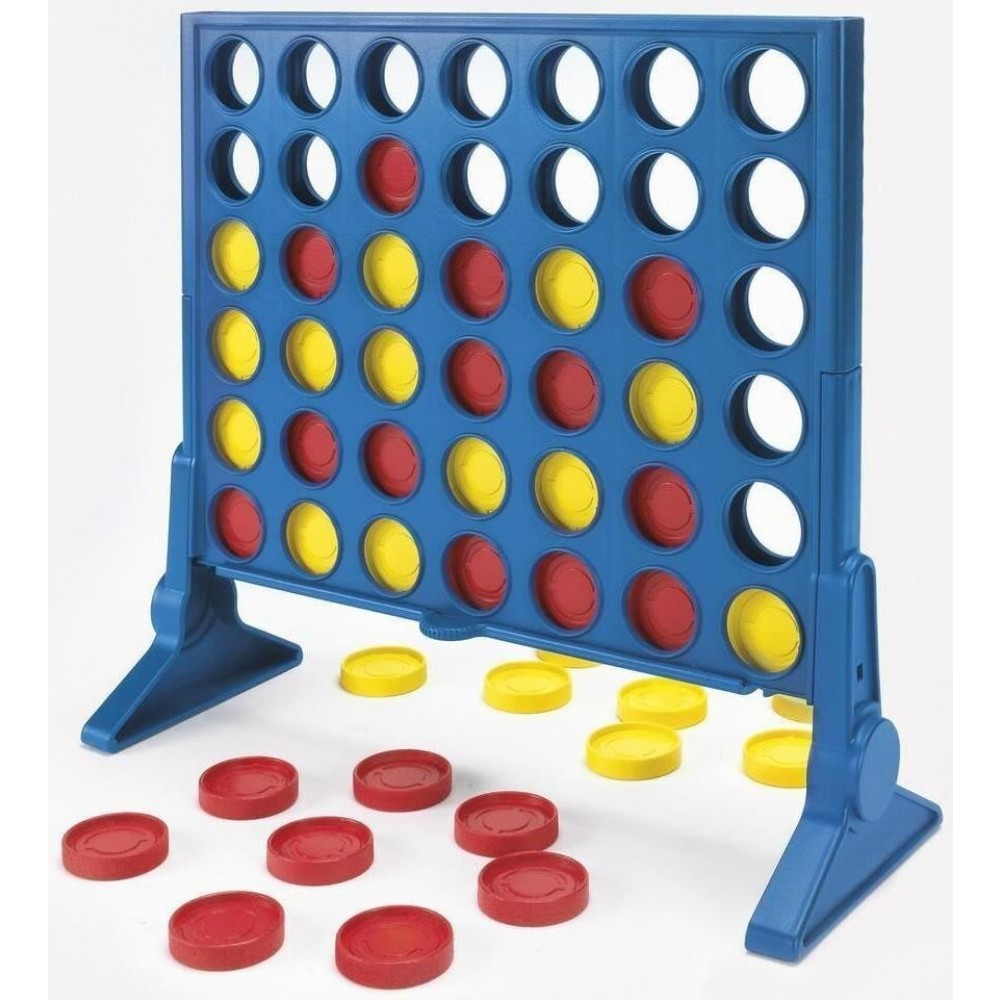
\includegraphics[width=8cm]{ressources/puissance4.jpg}
        \captionof{figure}{\centering     Le \emph{Puissance 4} est un jeu de stratégie en duel.
        }
        \label{IMG}
    \end{center}

\end{frame}
\begin{frame}
    \frametitle{}

    \begin{framed}
        \centering Comment construire un projet?
    \end{framed}

\end{frame}
\section{Identifier les besoins}
\begin{frame}
    \frametitle{Identifier les besoins}

    \begin{aretenir}[]
        Il s'agit de définir les \textbf{spécifications} du jeu.
    \end{aretenir}
\end{frame}
\begin{frame}
    \frametitle{}

    \begin{itemize}
        \item une grille de 7 colonnes et 6 lignes,
        \item 2 joueurs en alternance (rouge et jaune),
        \item gagnant: 4 pions horizontaux ou verticaux.
    \end{itemize}
    \begin{aretenir}[Remarque]
        Dans cette activité on construira une version simplifiée du jeu: on ne regardera pas les pions alignés en diagonal.
    \end{aretenir}
\end{frame}
\section{Modéliser}
\begin{frame}
    \frametitle{Modéliser - conception générale}

    \begin{aretenir}[]
        Il s'agit de définir un \textbf{algorithme général} du jeu.
    \end{aretenir}
    \begin{activite}
        Construire un déroulé du jeu.
    \end{activite}
\end{frame}
\begin{frame}
    \frametitle{Correction}
    Initialiser la grille\\
    Choisir un joueur de départ.\\
    Tant qu'il n'y a pas de gagnant:
    \begin{itemize}
        \item Demander la colonne choisie.
        \item Vérifier que la colonne n'est pas pleine.
        \item Placer le jeton en le \emph{laissant tomber} dans la colonne.
        \item Vérifier si le placement est gagnant:
              \begin{itemize}
                  \item si oui: partie terminée,
                  \item si non: changement de joueur.
              \end{itemize}
    \end{itemize}

\end{frame}
\begin{frame}
    \frametitle{Conception détaillée}

    \begin{aretenir}[]
        Il s'agit de donner les \textbf{signatures} des fonctions nécessaires.
    \end{aretenir}

\end{frame}
\begin{frame}
    \frametitle{}
    \textbf{Initialiser} la grille\\
    Choisir un joueur de départ.\\
    Tant qu'il n'y a pas de gagnant:
    \begin{itemize}
        \item \textbf{Demander} la colonne choisie.
        \item \textbf{Vérifier} que la colonne n'est pas pleine.
        \item \textbf{Placer} le jeton en le \emph{laissant tomber} dans la colonne.
        \item \textbf{Vérifier} si le placement est gagnant:
              \begin{itemize}
                  \item si oui: partie terminée,
                  \item si non: changement de joueur.
              \end{itemize}
    \end{itemize}
    \begin{activite}
        Donner une signature pour chaque étape de l'algorithme.
    \end{activite}

\end{frame}
\begin{frame}
    \frametitle{Correction}
    {\Large \textbf{\texttt{initialiser\_grille}}}
    \begin{itemize}
        \item rôle: construire la grille du jeu
        \item paramètres:
        \begin{itemize}
            \item nb\_col: entier
            \item nb\_lig: entier
        \end{itemize}
        \item renvoi: tableau de tableaux
    \end{itemize}

\end{frame}
\begin{frame}
    \frametitle{Correction}

    {\Large \textbf{\texttt{choisir\_colonne}}}
    \begin{itemize}
        \item rôle: demande la colonne où poser le jeton
        \item paramètres: aucun
        \item renvoi: la colonne choisie
    \end{itemize}

\end{frame}
\begin{frame}
    \frametitle{Correction}

    {\Large \textbf{\texttt{est\_remplie}}}
    \begin{itemize}
        \item rôle: vérifie si la colonne est remplie jusqu'en haut
        \item paramètres:
        \begin{itemize}
            \item grille: tableau
            \item colonne: entier
        \end{itemize}
        \item renvoi: booléen, vrai si la colonne est remplie
    \end{itemize}

\end{frame}
\begin{frame}
    \frametitle{Correction}

    {\Large \textbf{\texttt{placer\_jeton}}}
    \begin{itemize}
        \item rôle: place le jeton 
        \item paramètres:
        \begin{itemize}
            \item grille: tableau
            \item colonne: entier
        \end{itemize}
        \item renvoi: entier, la ligne où le jeton est placé
    \end{itemize}

\end{frame}
\begin{frame}
    \frametitle{Correction}

    {\Large \textbf{\texttt{verif\_gagnant}}}
    \begin{itemize}
        \item rôle: place le jeton 
        \item paramètres:
        \begin{itemize}
            \item grille: tableau
            \item joueur: entier
            \item ligne: entier
            \item colonne: entier
        \end{itemize}
        \item renvoi: booléen, vrai si le joueur a gagné
    \end{itemize}

\end{frame}
\begin{frame}
    \frametitle{}

    \begin{aretenir}[Remarque]
    Il sera peut-être nécessaire d'écrire d'autres fonctions  \emph{internes} pour exécuter certaines tâches, rendre le code plus lisible\dots
    \end{aretenir}

\end{frame}
\section{Implémenter}
\begin{frame}
    \frametitle{Implémenter}

    \begin{aretenir}[]
    Il s'agit de \textbf{transformer en code informatique} l'algorithme modélisé.
    \end{aretenir}

\end{frame}
\begin{frame}
    \frametitle{}

    \begin{activite}
    \begin{enumerate}
        \item Télécharger et extraire le dossier compressé \textbf{\texttt{puissance4-annexe.zip}} sur le site \url{https://cviroulaud.github.io}
        \item Ouvrir le fichier \textbf{\texttt{puissance4.py}}
    \end{enumerate}
    \end{activite}

\end{frame}
\begin{frame}
    \frametitle{}

    Le programme principal implémente l'algorithme général.

\end{frame}
\begin{frame}[fragile]

    \begin{center}
    \begin{lstlisting}[language=Python , basicstyle=\ttfamily\small, xleftmargin=2em, xrightmargin=2em]
grille = initialiser_grille()
joueur = ROUGE
\end{lstlisting}
    \captionof{code}{Initialisation}
    \end{center}
\begin{aretenir}[Remarque]
La couleur (\textbf{\texttt{ROUGE}}) du joueur est stockée dans une \textbf{constante}.
\end{aretenir}
\end{frame}
\begin{frame}[fragile]

    \begin{center}
    \begin{lstlisting}[language=Python , basicstyle=\ttfamily\small, xleftmargin=2em, xrightmargin=2em]
remplie = True
while remplie:
    colonne = choisir_colonne()
    remplie = est_remplie(grille, colonne)
\end{lstlisting}
    \captionof{code}{Demander la colonne et vérifier}
    \end{center}
\begin{aretenir}[Remarque]
Il faut initialiser la variable \textbf{\texttt{remplie}}.
\end{aretenir}
\end{frame}
\begin{frame}[fragile]

    \begin{center}
    \begin{lstlisting}[language=Python , basicstyle=\ttfamily\small, xleftmargin=2em, xrightmargin=2em]
ligne = placer_jeton(grille, colonne, joueur)
\end{lstlisting}
    \captionof{code}{Placer le jeton}
    \end{center}
\begin{aretenir}[Remarque]
On récupère la valeur de la \textbf{\texttt{ligne}}.
\end{aretenir}
\end{frame}
\begin{frame}[fragile]

    \begin{center}
    \begin{lstlisting}[language=Python , basicstyle=\ttfamily\small, xleftmargin=1em, xrightmargin=0em]
if verif_gagnant(grille, joueur, ligne, colonne):
    gagnant = True
else:
    # au tour de l'autre joueur
    joueur = changer_joueur(joueur)
\end{lstlisting}
    \captionof{code}{Vérifier le gagnant}
    \end{center}
\end{frame}
\begin{frame}
    \frametitle{}

    \begin{aretenir}[Remarques]
    
        \begin{itemize}
            \item Le code est découpé en fichiers puis en fonctions.
            \item Le programme principal est simplifié au maximum.
            \item La partie \emph{graphique} est pour l'instant hors programme.
        \end{itemize}
    \end{aretenir}

\end{frame}
\begin{frame}
    \frametitle{}

    \begin{activite}
    \begin{enumerate}
        \item Ouvrir le fichier \textbf{\texttt{constantes.py}}. Il contient des variables utilisables dans tout le programme. Elles ne doivent pas être modifiées.
        \item Ouvrir le fichier \textbf{\texttt{fonctions\_placement.py}}
        \item Compléter la fonction \textbf{\texttt{initialiser\_grille}} en construisant la grille par compréhension.
        \item Compléter la fonction \textbf{\texttt{est\_remplie}} qui vérifie si la colonne est remplie.
    \end{enumerate}
    \end{activite}
\end{frame}
\begin{frame}[fragile]
    \frametitle{Correction}

\begin{center}
\begin{lstlisting}[language=Python , basicstyle=\ttfamily\small, xleftmargin=1em, xrightmargin=0em]
def initialiser_grille() -> list:
    """
    construire la grille du jeu

    Returns:
        list: un tableau de HAUTEUR lignes et LARGEUR colonnes
    """
    return [[VIDE for i in range(LARGEUR)] for j in range(HAUTEUR)]
\end{lstlisting}
\captionof{code}{Initialiser}
\label{CODE}
\end{center}  

\end{frame}
\begin{frame}[fragile]
    \frametitle{}
\begin{center}
\begin{lstlisting}[language=Python , basicstyle=\ttfamily\small, xleftmargin=1em, xrightmargin=-.5em]
def est_remplie(grille: list, colonne: int) -> bool:
    """
    vérifie si la colonne est remplie jusqu'en haut

    Args:
        grille (list): le jeu
        colonne (int): la colonne

    Returns:
        bool: True si la colonne est remplie
    """
    # il suffit de vérifier si l'emplacement le plus haut est vide
    return not(grille[0][colonne] == VIDE)
\end{lstlisting}
\captionof{code}{Colonne remplie?}
\label{CODE}
\end{center}
    

\end{frame}
\begin{frame}
    \frametitle{}

    \begin{activite}    
        \begin{enumerate}
            \item Pour placer le jeton on écrit une fonction intermédiaire: \textbf{\texttt{tomber\_ligne(grille: list, colonne: int) $\rightarrow$ int}}. Elle renvoie la position du jeton qui est tombé.
            \item En utilisant la fonction précédente, compléter la fonction \textbf{\texttt{placer\_jeton}}
        \end{enumerate}
    \end{activite}

\end{frame}
\begin{frame}[fragile]
    \frametitle{Correction}

\begin{center}
\begin{lstlisting}[language=Python , basicstyle=\ttfamily\small, xleftmargin=1em, xrightmargin=-1em]
def tomber_ligne(grille: list, colonne: int) -> int:
    ligne = 0
    while ligne < HAUTEUR and grille[ligne][colonne] == VIDE:
        # on descend tant qu'on n'est pas en bas ou sur une case remplie
        ligne = ligne + 1

    # renvoie la dernière place vide
    return ligne-1
\end{lstlisting}
\captionof{code}{Trouve la ligne d'arrivée}
\label{CODE}
\end{center}    

\end{frame}
\begin{frame}[fragile]
    \frametitle{}

\begin{center}
\begin{lstlisting}[language=Python , basicstyle=\ttfamily\small, xleftmargin=.5em, xrightmargin=-4.5em]
def placer_jeton(grille: list, colonne: int, joueur) -> int:
    ligne = tomber_ligne(grille, colonne)
    grille[ligne][colonne] = joueur
    return ligne
\end{lstlisting}
\captionof{code}{Place le jeton}
\label{CODE}
\end{center}   

\end{frame}
\begin{frame}
    \frametitle{}

\begin{activite}
Étude du reste du code:
\begin{enumerate}
    \item Comment fonctionne la fonction \textbf{\texttt{verif\_gagnant}}?
    \item Dans la fonction \textbf{\texttt{verif\_verticale}}, quelles sont les conditions pour que la boucle \textbf{\texttt{while}} soit exécutée?
    \item Que faut-il ajouter pour vérifier les diagonales?
\end{enumerate}
\end{activite}

\end{frame}
\begin{frame}[fragile]
    \frametitle{Correction}

    \begin{center}
    \begin{lstlisting}[language=Python , basicstyle=\ttfamily\small, xleftmargin=.5em, xrightmargin=-1.5em]
if verif_verticale(grille, joueur, ligne, colonne) or \
    verif_horizontale_droite(grille, joueur, ligne, colonne) or \
    verif_horizontale_gauche(grille, joueur, ligne, colonne):
\end{lstlisting}
    \captionof{code}{Gagnant?}
    \label{CODE}
    \end{center}
Pour gagner il suffit (\textbf{\texttt{or}}) qu'une des conditions soient vérifiée.
\end{frame}
\begin{frame}[fragile]
    \frametitle{Correction}
\begin{aretenir}[Remarque]
Pour vérifier si la partie est gagnée il suffit de regarder \emph{vers le bas} de la grille.
\end{aretenir}
    \begin{center}
    \begin{lstlisting}[language=Python , basicstyle=\ttfamily\small, xleftmargin=2em, xrightmargin=2em]
while ligne < HAUTEUR and 
        grille[ligne][colonne] == joueur and 
        compteur < 4:
\end{lstlisting}
    \end{center}
\begin{itemize}
    \item on ne sort pas de la grille,
    \item les jetons sont de la même couleur,
    \item on n'a pas encore 4 jetons de même couleur.
\end{itemize}
\end{frame}
\begin{frame}[fragile]
    \frametitle{}

    Pour améliorer le jeu il faut:
    \begin{itemize}
        \item créer les fonctions \textbf{\texttt{verif\_diagonale}},
        \item modifier la condition de la fonction \textbf{\texttt{verif\_gagnant}}.
    \end{itemize}
    \begin{center}
    \begin{lstlisting}[language=Python , basicstyle=\ttfamily\small, xleftmargin=.5em, xrightmargin=-1.5em]
if verif_verticale(grille, joueur, ligne, colonne) or \
    verif_horizontale_droite(grille, joueur, ligne, colonne) or \
    verif_horizontale_gauche(grille, joueur, ligne, colonne) or \
    verif_diagonale(grille, joueur, ligne, colonne):
\end{lstlisting}
        \end{center}
\end{frame}
\end{document}